\documentclass[border=4pt]{standalone}
\usepackage{tikz}
\usetikzlibrary{arrows,positioning}
\begin{document}
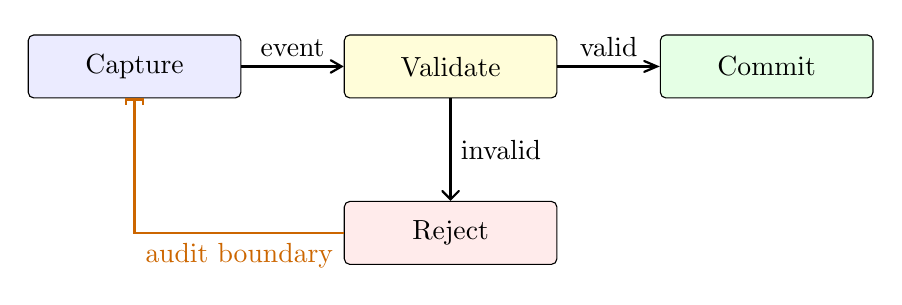
\begin{tikzpicture}[
  node distance=13mm,
  stage/.style={draw,rounded corners=2pt,minimum width=27mm,minimum height=8mm,align=center},
  flow/.style={line width=.8pt,-{angle 60}}
]
  \node[stage,fill=blue!8] (capture) {Capture};
  \node[stage,fill=yellow!15,right=of capture] (validate) {Validate};
  \node[stage,fill=green!10,right=of validate] (commit) {Commit};
  \node[stage,fill=red!8,below=of validate] (reject) {Reject};

  \draw[flow] (capture) -- node[above]{event} (validate);
  \draw[line width=.8pt,-{angle 45}] (validate) -- node[above]{valid} (commit);
  \draw[line width=.8pt,-{angle 90}] (validate) -- node[right]{invalid} (reject);
  \draw[orange!80!black,line width=.8pt,-{square bracket}]
    (reject.west) -| node[pos=.25,below]{audit boundary} (capture.south);
\end{tikzpicture}
\end{document}
